\subsection{Touch Circuit of C. elegans}
\label{section: touch-circuit}

Any such kind of complete circuit would consists of neurons from all 3 categories: sensory neuron, inter-neuron and motor neuron in order to facilitate an observable and
meaningful behavior.

The touch circuit is identified in Chalfie et al. \cite{chalfie_neural_1985}, using laser ablation techniques to kill the precursors of the neuron cells (mostly in
embryos except AVM) and observe its effect on the touch sensitivity of C. elegans.

\subsubsection{Classification}
\paragraph{Sensory input}
There are 6 touch receptor cells:
\begin{itemize}
  \item \emph{ALMR, ALML}: anterior lateral microtubule cells. They are required for a full response to touch on the head.
  \item \emph{PLMR, PLML}: posterior lateral microtubule cells. They are required for any response to touch on the tail.
  \item \emph{AVM}: anterior ventral microtubule cell. AVM alone mediates a very weak touch response to head touch.
  \item \emph{PVM}: posterior ventral microtubule cell. PVM alone does not mediate a detectable touch response.
\end{itemize}

\paragraph{Motor output} 
Sets (coupled by gap junctions) of ventral cord motor neurons are responsible for muscle cell activity: \cite{white_structure_1986}
\begin{itemize}
  \item \emph{A motor neurons} (12 VA cells and 9 DA cells)
  \item \emph{B motor neurons} (11 VBs and 7 DBs)
  \item \emph{D motor neurons} (13 VDs and 6 DDs)
  \item \emph{11 AS motor neurons} share many of the properties of the DA cells
\end{itemize}
A and B neuron cells mediate muscle contraction for backward and forward movement (excitatory), and D cells mediate contralateral inhibition.

From Chalfie et al. \cite{chalfie_neural_1985}, but there is no mention of whether all the A, B, D, AS neurons involve in touch response behavior.

\subsubsection{Data}
From the synapsis data, only 4 pairs of interneurons AVA, AVB, PVC, AVD synapse onto the motor neurons of the ventral cord and span the full length of the cord. They form synapses with touch
cells in an interestingly complementary pattern:

\begin{tabular}{| l | l l |}
  \hline
  \multirow{2}{*}{Interneurons} & \multicolumn{2}{| c |}{Synapses made by} \\ \cline{2-3}
    & Anterior touch receptors & Posterior touch receptors \\ \hline
  AVA & - & chemical \\
  AVB & chemical(only AVM) & - \\
  PVC & chemical & gap \\
  AVD & gap & chemical \\
  \hline
\end{tabular}


\subsubsection{Testing}

\paragraph{Speculation} Is there a relationship between the multiplicity and type of synapses and the effectiveness of that neuron pathway.

Example (Chalfie et al. Figure 4):

The figure below shows that the anterior touch cells (ALM \footnote{AVM not developed in young larvae with which this experiment is carried out}) make EJ with AVA and
AVD, and CJ with PVC; posterior touch cells (PLM) make EJ with PVC, and Chemical with AVD. 
The laser ablation experiment shows that AVA and AVD has no effect on anterior sensitivity, and PVC has no effect on posterior sensitivity. Hence it seems that the gap
junction synapses between sensory and interneurons are more important in this touch circuit.

In contrast, the chemical synapses seem to play an inhibitory role. For example, the Chemical from ALM/AVM to PVC seems to inhibit the neuron signal to be propagated to B
motor neurons, which will cause an inappropriate response.

Data fitting might be able to model the effectiveness of signal propagation in these circuits. In addition to setting a $\tau$ for weight (multiplicity), the type of
synapses could also be taken into account.

Also, lots of connections such as the reciprocal synapses between AVA and PVC are not explained fully in terms of neurology. They might enable/inhibit certain pathways
for certain behavior to be effective. (eg. reaction time)

\paragraph{Rewiring} It seems to me that rewiring could occur as adaptation for C elegans. For C elegans in postembryonic stage, when AVD is killed, they regain some
touch sensitivity after a few more touches, which suggest that the Chemical between AVM-AVB-AVA-AVD \footnote{from experimental results AVA seems to be important in this
alternative pathway} might act as an alternative pathway, which is not the optimum, but might be in
use when the optimum path is damaged.

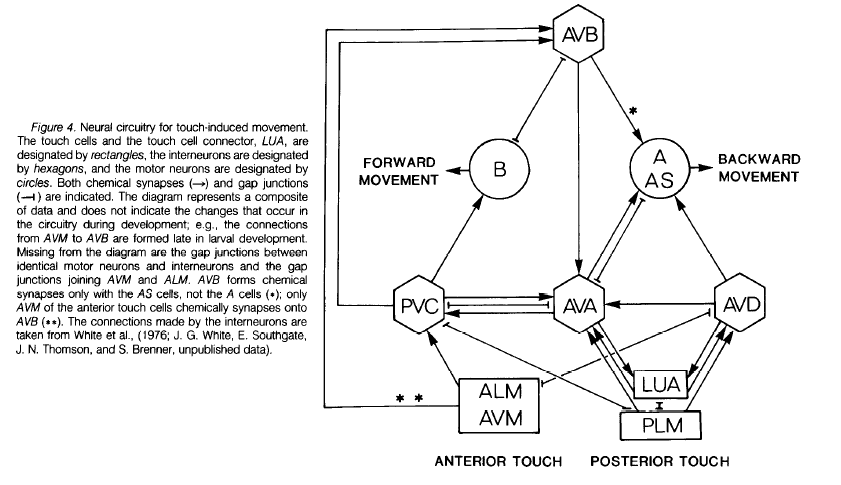
\includegraphics[scale=0.8]{graphics/TouchCircuit}

The following table illustrates the result of disabling certain interneuron(s):

\begin{tabular}{| l | l l l l l l |}
  \hline
  \multirow{2}{*}{Interneurons killed} & \multicolumn{2}{ c }{Sensitive at head} & \multicolumn{2}{ c }{Sensitive at tail}
    & \multirow{2}{*}{Forward movement} & \multirow{2}{*}{Backward movement} \\ \cline{2-3} \cline{4-5}
    & Larva & Adult & Larva & Adult & \\
  PVC & \checkmark & \checkmark & - & - & \checkmark & \checkmark \\
  AVD & - & \checkmark (adapted) & \checkmark & \checkmark & \checkmark & \checkmark \\
  AVD, AVM & - & - & \checkmark & \checkmark & \checkmark & \checkmark \\
  AVA & \checkmark & \checkmark & \checkmark & \checkmark & \checkmark & uncoordinated \footnote{uncoordinated when moving in the indicated direction and when stopping
after moving in the opposite direction} \\
  AVA, AVD & - & \checkmark \footnote{Anterior touch could not make them move backward, but could stop them if they were moving forward. The touch also stopped
pharyngeal pumping} & \checkmark & \checkmark & \checkmark & - \\
  AVB & \checkmark & \checkmark & \checkmark & \checkmark & uncoordinated & \checkmark \\
  AVB, PVC & \checkmark & \checkmark & - & - & - \footnote{incapable of propagating a wave of muscle contraction for forward motion in the body, but did move forward
from waves generated in the head} & \checkmark \\
  \hline
\end{tabular}

\subsection{Other functional circuits suggested}

All these circuits could be the biological ground truth for doing clustering. Checking 1D eigenspace would be simple. 3D needs more thoughts.

\newpage

\begin{figure}[h!]
  \caption{Learned NaCl Aversion. Based on data from Hukema et al.(2006), Tomioka et al. (2006), Fu et al. (2009), Kano et al. (2008), Ishihara et al. (2002), and White et al. (1986)}
  \centering
  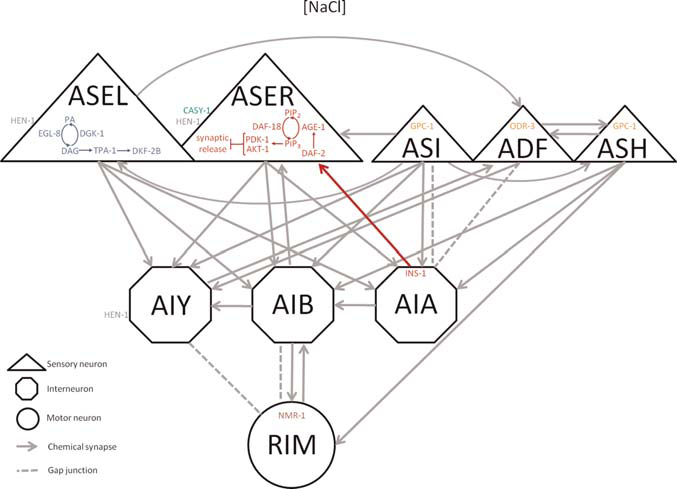
\includegraphics[scale=0.8]{graphics/LearnedNaClAversion}
  \label{fig:NaCl_aversion}
\end{figure}

\begin{figure}[H]
  \paragraph{Electrosensory Behavior \cite{gabel_neural_2007} }
  It is the biological ability to perceive natural electrical stimuli.

  The following diagram is not considered as comprehensive, but the author did suggest why interneurons such as AIY are not significant in electrosensory neural circuits
according to the experiments.

  \centering
  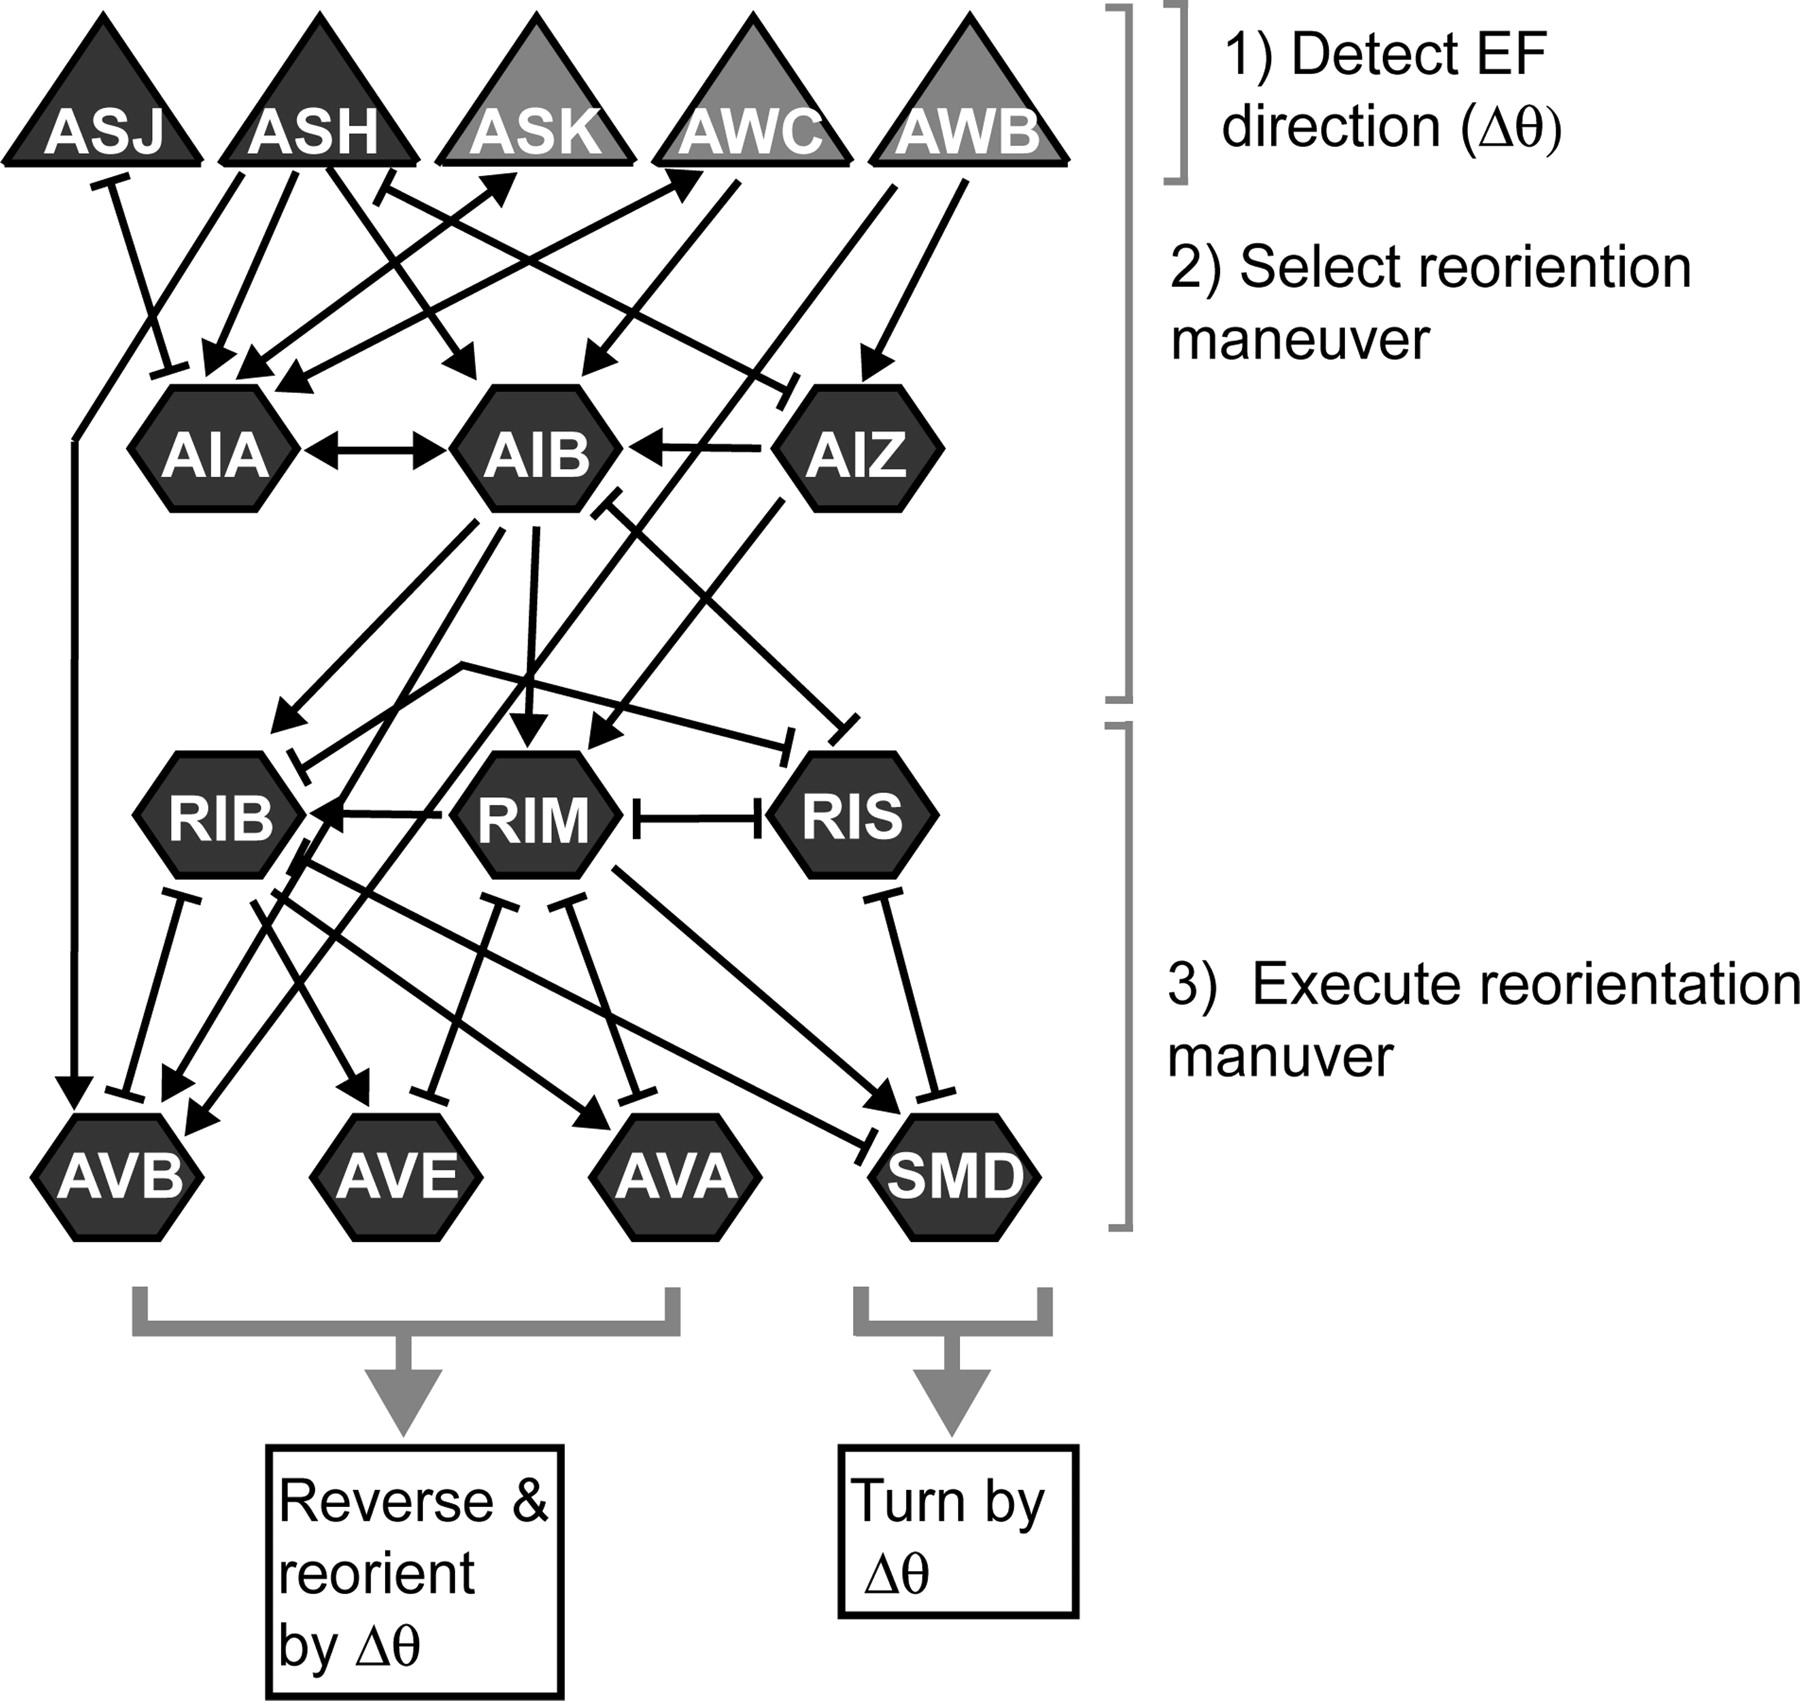
\includegraphics[scale=0.25]{graphics/ElectroSensoryCircuit}
  \label{fig:electro_sensory}
  \caption{Neural circuits for electrosensory behavior. The wiring diagram of neural pathways that might contribute to electrosensory behavior is shown. Synaptic connections
between neurons follow the wiring diagram established by White et al. (1986). Sensory neurons are indicated by red triangles. Interneurons and command motor neurons are
indicated by hexagons. Chemical synaptic connections between neurons are indicated by arrows. Gap junctions are indicated by brackets. We suggest that the primary
neurons for electrosensory detection are ASJ and ASH. RIM and AVA appear contribute to turns and reversals during electrosensory steering, respectively. Additional
neurons show pathways that might connect ASJ, ASH, RIM, and AVA to motor output during electrosensory behavior, as well as several other neurons that have been
implicated in the execution of turns and reversals during exploratory behaviors (Tsalik and Hobert, 2003; Wakabayashi et al., 2004; Gray et al., 2005). EF, Electric
field. sed on data from Hukema et al.(2006), Tomioka et al. (2006), Fu et al. (2009), Kano et al. (2008), Ishihara et al. (2002), and White et al. (1986)}
\end{figure}


